\lecture{Operating Systems - Introduction}{2023-03-13}{16:00}{Farzad}{RB LT1}

\section*{Development of Operating Systems}

\subsection*{Late 1940s}
There were no operating systems, the programmer was also the user. Programs and data were entered in binary through switching switches on the front of the machine (each switch represented one bit). Output was given through lights (each light represented one bit). The programmer did everything that an operating system does today.

\subsection*{1950s}
Specialist operators were introduced. These people are not programmers. They tend to the machine, feed the programs to the machine and deliver back to the output.

Programmers use punch machines to encode their programmer as a series of holes in stiff cards. Computers can read and interpret the holes in the punch cards.

The operators acted as an human interface between the programmer and the hardware. 

\subsection*{1960s}
The need for a human (to load and unload punched cards, starting and stopping devices) added delay into the system. 

The programmers now punched instructions onto control cards which were inserted at the appropriate places before and after the program cards and data cards

The commands were written in specially developed job control languages. 

\subsection*{Late 1960s and 1970s}
Computer users found that programs were growing in size and required more memory. The initial solution was to break programs up into small chunks, each fitting in the available memory.

We now have larger memories, however we need to timeshare this between different programs.

The issue of protecting one program from another became more and more important. This is a task which the OS performs. 

\subsection*{1980s}
Computers now have the ability to communicate with one another. 

\subsection*{1990s}
Previously, operating systems have been developed specifically for particular hardware platforms (for example, MS-DOS for the PC).

This move allowed generic operating systems (for example Linux) to run on any hardware. 

\section*{What Is An Operating System?}
The \textit{Operating System} sits between the application and the hardware. I allows the application to interface with the hardware, so that there is only one thing interfacing with the hardware. The users interface with the applications, and at times the operating system.

Operating systems, at heart, are computer programs. They are written, tested and compiled just like any other program. Operating systems will begin running as soon as the computer has turned on, this usually happens automatically. 

The operating system makes the hardware more useful and user friendly.

\section*{What Does The Operating System Do?}
Operating systems provide an environment which helps other programs do productive work; helps the user to develop \& run programs, by providing a convenient environment; and starts and stops applications by sharing the CPU between them.

The operating system is also responsible for managing memory, this involves keeping track of which parts of memory are in use and which are free; and providing a mechanism by which applications can ask for more memory to be allocated to them or give back memory which they no longer need.

The operating system handles inputs and outputs; differences between hardware devices (so that all applications can interface with hardware the same); and controlling input/ output and processing so that they can happen at the same time.

The operating system also provides data management, which involves managing the different physical drives and how to move data between them; protection to the CPU of overlapping processes; networking support through covering up differences between machines; and error handling \& recovery which provides a way for the user to interface with errors. 

\section*{Operating System Interfaces}
The operating system can be interfaced with in a number of ways. This includes through a Graphical User Interface - where icons and pictures are used to control what happens in the OS or through a Command Interpreter - where text commands are entered at a prompt which the operating system interprets.

Modern operating systems will come with both a GUI and command interpreter.

The GUI, command interpreter and application programs don't directly interface with the operating system. They all interface with the system services, which provide a set of functions which request services of the operating system.

\section*{Kernel}
The \textit{kernel} is the central component (the heart) of an operating system. It interfaces between hardware components and software applications - this means it males the software interact with the hardware to get a specific task done. 

The kernel decides the amount of resources (RAM, GPU, etc) to be used by every application and the order of execution of programs. The kernel has a separate memory space so that its functions are independent (this is the bit of memory, both primary and secondary, which isn't listed as usable in OS). 

The kernel is the central authority which guides memory and keeps an eye on all the hardware and software data flow. The kernel responds to system calls - which are calls where processes can demand resources. 
\subsection*{CPU Operation Modes}
There are two modes of CPU operation, each of which have different limitations on instructions.

By default, machines run in user mode; when it wants to do something special, it has to change into kernel mode. 
\subsubsection*{User Mode}
The CPU can only execute a subset of its instructions - the more common ones (add, subtract, load, store, etc). When a program is executed, it doesn't have access to memory, hardware and such resources.
\subsubsection*{Kernel Mode}
The CPU can execute all of its instructions, including extra privileged instructions. When a program is executed, it has direct access to memory, hardware and such resources.

\subsection*{Types of Kernel}
\begin{figure}[H]
    \centering
    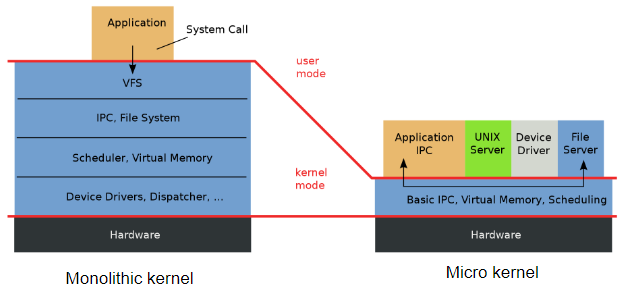
\includegraphics[width=0.6\textwidth]{assets/kernel-types.png}
\end{figure}
\subsubsection*{Monolithic Kernel}
Both the user services and kernel services are kept in the same address space (this means the entire OS is in the kernel space). It is larger than micro kernel, less access time and fast execution, hard to extend. It has higher performance, however higher risk of a systems crash.

Linus uses the monolithic kernel.

\subsubsection*{Microkernel}
The user services and kernel services are kept in separate address spaces. This means the kernel is smaller in size, there is minimum code in kernel space, greater access time with slow execution. It is easily extendible and has lower responsibility.

Windows uses a hybrid of the two types of kernel.

\section*{Types of Operating System}
Different types of operating system are required for different purposes.
\subsection*{Batch Systems}
These were the earliest systems developed. Data and commands to manipulate the program and data are all submitted together to the computer in the form of a \textit{job}. There is little-to-no interaction between the users and an executing program.

These systems are used where there is no need for operator intervention once the job has started, for example in payroll processing or bank/ credit card statement generation. 

\subsection*{Interactive Systems}
The most common mode of using a computer is through using a keyboard, mouse and screen.

Interactive systems are a significant improvement over \textit{batch systems} as it is now possible to intervene directly while a program is being developed or as it is running. Single user interactive systems are available, these provide multitasking and interactive computing on a single-user basis such as Windows, MS-DOS and OS/2. Also, multi user interactive systems are available, these provide interactive computing on a multi-access or multi-user basis (using different terminals) such as Unix, Linux, Windows 10, Ubuntu, Mac OS. 

\subsection*{General Purpose}
A given environment may want a bit of everything - for example a timesharing system may support interactive users and also include the ability to run programs in batch mode.

\subsection*{Network}
To share resources such as printers and databases across a network, such as Windows NT Server.

\subsection*{Distributed}
The most recent development in operating systems, this meets the requirements of a multi-user system. It consists of a group of machines acting together as one. When a user starts a program, it may run on the local machine.However if that computer is heavily loaded and the operating system knows that another machine is idle then the job may be transferred to that idle machine.

\subsection*{Specialist}
Dedicated to processing large volumes of data which are maintained in an organized way such as a real-time operating system would require for example a banking system. 

\section*{Design of Operating Systems}
An operating system is a very large piece of software. To design, build and maintain large software systems like this requires a high-level view of how the system is structured and how its different components work together. 